\documentclass[conference]{IEEEtran}

\usepackage{bm,cite,algorithm,algorithmic,float,amsmath,amssymb}

\usepackage{amssymb}
\usepackage{amsmath}
\usepackage{graphicx}
\usepackage{cite}
%\usepackage{citesort}
%\usepackage[utf8x]{inputenc}
\usepackage{amsthm}
\usepackage{framed}
\usepackage{url}
%\newtheorem{definition}{Definition}
\newtheorem{theorem}{Theorem}
\newtheorem{lemma}{Lemma}
\newtheorem{proposition}{Proposition}
\newtheorem{axiom}{Axiom}
\newtheorem{corollary}{Corollary}
\newtheorem{remark}{Remark}
\newtheorem{example}{Example}
\newtheorem{property}{Property}
\newtheorem{definition}{Definition}
\newtheorem{hypothesis}{Hypothesis}
%\bibliographystyle{IEEEtran}
\IEEEoverridecommandlockouts

\newcommand{\defequal}{\mbox{$\stackrel{\triangle}{=}$}}

\usepackage{graphicx,epstopdf}
\usepackage{epsfig}	
\usepackage{amsfonts}
%\usepackage{bbm}
\floatname{algorithm}{Algorithm}
\newcommand{\EX}[1]{\mathbb{E}\left\{{#1}\right\}}
\newcommand{\EXs}[2]{\mathbb{E}_{{#1}}\left\{{#2}\right\}}
\newcommand{\PDF}[2]{f_{{#1}}\left({#2}\right)}
\newcommand{\CDF}[2]{F_{{#1}}\left({#2}\right)}
\newcommand{\CCDF}[2]{C_{{#1}}\left({#2}\right)}
% for binomial coefficients (AmS-LaTeX)
%\newcommand{\bc}[2]{\genfrac{(}{)}{0pt}{}{#1}{#2}}
\newcommand{\bc}[2]{{}_{#1}C_{#2}}
\newcommand{\BG}[2]{\bar{{#1}}_{{#2}}}
\newcommand{\TG}[1]{\tilde{{#1}}}

\newcommand{\A}[1]{(\textbf{A#1:})}

%\newcounter{mytempeqncnt}

\DeclareMathOperator*{\argmax}{argmax}
\DeclareMathOperator*{\argmin}{argmin}

\hyphenation{op-tical net-works semi-conduc-tor}
\raggedbottom
\begin{document}
	
	\title{Goal-Oriented $1$-Bit Quantization with Uncertain Goals\thanks{M. Egan is with Univ Lyon, INRIA, INSA Lyon, CITI, France (email: malcolm.egan@inria.fr)}}
	
	% for a Family of Non-Separable Distortion Criteria}

\author{Malcolm Egan}
%{$^1$\footnotesize INSA}\\
%{$^2$\footnotesize INRIA}\\
%{$^3$\footnotesize Faculty of Electrical Engineering, Czech Technical University in Prague}}

\maketitle

\begin{abstract}

\end{abstract}


\maketitle

\section{Introduction}



\section{Problem Formulation}

Consider a data source $P_{\mathbf{X}}$ with data $\mathbf{X} \in \mathbb{R}^d,~d \geq 1$. A $1$-bit quantizer of $\mathbf{X}$ consists of a reproduction set $\mathcal{Y} = \{\mathbf{y}_1,\mathbf{y}_2\} \subset \mathbb{R}^d$ and the quantizer function $Q:\mathbb{R}^d \rightarrow \mathcal{Y},~\mathbf{x} \mapsto \hat{\mathbf{x}}$. 

The distortion in the quantizer is measured via $D: \mathbb{R}^d \times \mathbb{R}^d \rightarrow \mathbb{R}_+$. A standard choice of the distortion function is the Euclidean square error $D_{\mathrm{SE}}(\mathbf{x},\hat{\mathbf{x}}) = \|\mathbf{x} - \hat{\mathbf{x}}\|^2,~\mathbf{x},\hat{\mathbf{x}} \in \mathbb{R}^d$. The performance criterion for the quantizer is then defined as 
\begin{align}
\mathcal{E} = \mathbb{E}[D(\mathbf{X},Q(\mathbf{X}))],
\end{align}
with the optimal quantizer given by
\begin{align}\label{eq:opt_expect}
\min_{\mathbf{y}_1,\mathbf{y}_2 \in \mathbb{R}^d} \mathbb{E}[D(\mathbf{X},Q(\mathbf{X}))].
\end{align}

The optimal quantizer is then specified by the source distribution $P_{\mathbf{X}}$ and the distortion function $D$. The problem of coping with an imperfectly specified $P_{\mathbf{X}}$ or $D$ is known as  mismatched quantization. In the case the distortion function is unknown, a common problem is to characterize the performance loss when the quantizer is designed based on $D_{\mathrm{SE}}$. 

In this paper, we address the question: \textit{is there a better design criterion for $1$-bit quantization with an imperfectly specified distortion function?}    

\section{Impact of Uncertainty in the Distortion}

In order to understand the impact of uncertainty on performance, we consider two models of distortion functions. 

\subsection{Data-Weighted Distortion}

Given continuous data $\mathbf{X} \in \mathbb{R}^d$ with dependent elements admitting the joint density $p_{\mathbf{X}}$, the standard distortion criterion is given by 
\begin{align}
&\mathbb{E}[D_{\mathrm{SE}}(\mathbf{X},Q(\mathbf{X}))]\notag\\
&= \int_{\mathbb{R}^d} D_{\mathrm{SE}}(\mathbf{x},Q(\mathbf{x}))p_{\mathbf{X}}\mathrm{d}\mathbf{x}\notag\\
&= \int_{\mathbb{R}^d} D_{\mathrm{SE}}(\mathbf{x},Q(\mathbf{x})) C(F_1(x_1),\ldots,F_d(x_d))\prod_{i =1}^d p_{X_i}(x_i)\mathrm{d}\mathbf{x}.
\end{align}
Let $K(\mathbf{x}) = c(F_1(x_1),\ldots,F_d(x_d))$. Then,
\begin{align}
&\mathbb{E}_{\mathbf{X}}[D_{\mathrm{SE}}(\mathbf{X},Q(\mathbf{X}))]\notag\\
&= \mathbb{E}_{\tilde{\mathbf{X}}}[K(\mathbf{X})D_{\mathrm{SE}}(\tilde{\mathbf{X}},Q(\tilde{\mathbf{X}}))],
\end{align}
where $\tilde{X} \sim \prod_{i=1}^d P_{X_i}$; that is, the elements of $\tilde{\mathbf{X}}$ are independent. The function $c: [0,1]^d \rightarrow \mathbb{R}_+$ is known as the copula density function. 

Uncertainty in the dependence structure of $\mathbf{X}$ is captured via this distortion function. This suggests a useful distortion criterion in this setting is 
\begin{align}
D_K(\mathbf{X},Q(\mathbf{X})) = K(\mathbf{X})D_{\mathrm{SE}}(\mathbf{X},Q(\mathbf{X})).
\end{align}

\subsection{$p$-Error Distortion}

A common distortion function for post-training quantization of neural networks \cite{Nahshan2021loss} is the $p$-error, given by 
\begin{align}
D_p(\mathbf{X},\hat{\mathbf{X}}) = \sum_{i=1}^d |x_i - \hat{x}_i|^p,
\end{align}  
where $\hat{\mathbf{X}} = Q(\mathbf{X})$. 

\subsection{Impact of Distortion Uncertainty for Symmetric Quantizers}

To illustrate the impact of uncertainty in the data-weighted and $p$-error distortion functions, we consider the case of symmetric quantizers. We allow $\mathcal{Y} = \{-B,B\}$ for $B \in \mathbb{R}_+$. The quantization point is chosen via 
\begin{align}
Q(x) = \arg\min_{\hat{x} \in \{-B,B\}} (x - \hat{x})^2.
\end{align}

\begin{figure}
\centering
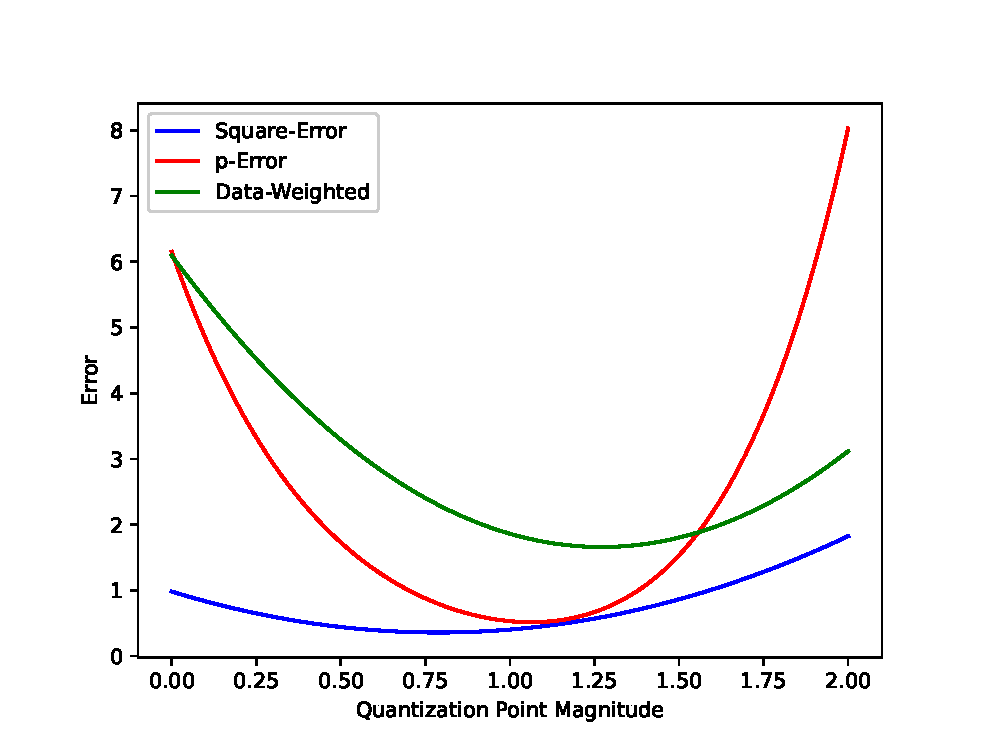
\includegraphics[width=\linewidth]{impact_distortion.eps}%{traces.eps}
\caption{Impact of distortion functions. $X \sim \mathcal{N}(0,1)$, $p = 5$, $K(x) = \exp(|x|)$.}
\label{fig:impact_distortion}
\end{figure}

Fig.~\ref{fig:impact_distortion} plots the impact on the true distortion metric for three scenarios. Observe that the optimal quantization point magnitude (i.e., $B$) is significantly different between the three scenarios. This suggests that utilizing a quantizer based on $D_{\mathrm{SE}}$ is undesirable. If the target distortion function is known, it can be utilized to construct a new quantizer. However, ...  

\section{Risk-Averse Quantization}

\subsection{Risk-Averse Criteria}

Suppose that $\mathcal{D}$ is a set of distortion functions $D: \mathbb{R}^d \times \mathbb{R}^d \rightarrow \mathbb{R}_+$ and $P_D$ is a prior distribution on $\mathcal{D}$. In this case, we seek to construct a quantizer solving
\begin{align}
\min_Q \mathbb{E}_{D,\mathbf{X}}[D(\mathbf{X},Q(\mathbf{X}))],
\end{align}
This is intractable in general. A standard approach is to first choose a reference distortion function $D_{\mathrm{ref}}$; e.g., 
\begin{align}
D_{\mathrm{ref}}(\mathbf{X},Q(\mathbf{X})) = \|\mathbf{X} - \hat{\mathbf{X}}\|^2.
\end{align}
The quantizer is then constructed via 
\begin{align}
\min_Q \mathbb{E}[D_{\mathrm{ref}}(\mathbf{X},Q(\mathbf{X}))].
\end{align}
While standard, this approach ignores any uncertainty in the distortion function. 

Fix the quantizer $Q$ and note that 
\begin{align}
\mathbb{E}_{D,\mathbf{X}}[D(\mathbf{X},Q(\mathbf{X}))] &= \mathbb{E}_D\left[\int_0^{\infty} \mathbb{P}(D(\mathbf{X},Q(\mathbf{X})) > u)\mathrm{d}u\right]\notag\\
&= \int_0^{\infty} \mathbb{E}_D\left[\mathbb{P}(D(\mathbf{X},Q(\mathbf{X})) > u)\right]\mathrm{d}u.
\end{align}
In order to account for uncertainty, we seek a conservative estimate of $\mathbb{E}_D\left[\mathbb{P}(D(\mathbf{X},Q(\mathbf{X})) > u)\right]$ for each $u \in [0,\infty)$. Let $h: [0,1] \rightarrow [0,1]$ be a concave function satisfying $h(0) = 0$ and $h(1) = 1$. We then have
\begin{align}
\mathbb{E}_D\left[\mathbb{P}(D(\mathbf{X},Q(\mathbf{X})) > u)\right] \leq \mathbb{E}_D\left[h\left(\mathbb{P}(D(\mathbf{X},\hat{\mathbf{X}}))\right)\right]. 
\end{align}
The final step (as applied in the expected distortion case) is to utilize the approximation
\begin{align}
\mathbb{E}_D\left[h\left(\mathbb{P}(D(\mathbf{X},\hat{\mathbf{X}}))\right)\right] \approx h\left(\mathbb{P}(D_{\mathrm{ref}}(\mathbf{X},\hat{\mathbf{X}}))\right).
\end{align}
The resulting quantity 
\begin{align}
\rho(D_{\mathrm{ref}}(\mathbf{X},Q(\mathbf{X}))) = \int_0^{\infty} h\left(\mathbb{P}(D_{\mathrm{ref}}(\mathbf{X},Q(\mathbf{X})))\right)\mathrm{d}u
\end{align}
is known as a \textit{distortion risk measure}. By increasing the nonlinearity of $h$, a greater level of uncertainty in $D$ can be accounted for. 

%An equivalent representation is 
%\begin{align}
%	\min_Q \sup_D \int_0^{\infty} \mathbb{P}(D(\mathbf{X},Q(\mathbf{X})) > u)\mathrm{d}u.
%\end{align} 
%Suppose we take a reference $D_{\mathrm{ref}} \in \mathcal{D}$. We can ask for a given $u$ and $D \in \mathcal{D}$, how $\mathbb{P}(D(\mathbf{X},Q(\mathbf{X})) > u)$ differs from $\mathbb{P}(D_{\mathrm{ref}}(\mathbf{X},Q(\mathbf{X})) > u)$. We impose the condition 
%\begin{align}
%	\mathbb{P}(D(\mathbf{X},\hat{\mathbf{X}}) > u) \leq h(\mathbb{P}(D_{\mathrm{ref}}(\mathbf{X},\hat{\mathbf{X}}) > u)),~u \in \mathbb{R}_+.
%\end{align}
%\textbf{TODO: Discuss the link with $\mathcal{D}$...} Another perspective is to assume there is a prior distribution on $D$. In this case, we seek to solve 
%\begin{align}
%	&\min_{Q} \mathbb{E}_{D,X}[D(X,\hat{X})]\notag\\
%	&= \min_Q \mathbb{E}_D\left[\mathbb{E}_X[D(X,\hat{X})]\right]
%\end{align}
%since $X$ and $D$ are presumably independent. We can write $\mathbb{E}_X[D(X,\hat{X})] = f(D)$. If differentiable we obtain 
%\begin{align}
%	&\mathbb{E}_D\left[\mathbb{E}_X[D(X,\hat{X})]\right]\notag\\
%	&\approx \mathbb{E}_D[f(D_{ref}) + f'(D_{ref})(D - D_{ref})].
%\end{align}
%So this probably doesn't help. I want to find an approximation where the risk measure picture naturally falls out. This must be known... 
%\begin{align}
%	\mathbb{E}[D(X,\hat{X})] = \int \mathbb{E}_D[\mathbb{P}(D(X,\hat{X}) > u)]\mathrm{d}u
%\end{align}
%So the idea is to replace the expectation with a function centered on one point. What if we had $\mathbb{E}[X] = \int xdF(x)$. We could use Holder's inequality: $\mathbb{E}[X] = \mathbb{E}[1\cdot X] \leq (\mathbb{E}[X^s])^{r/s}$. We would obtain the power distortion function by the approximation $X \approx x_{ref}$. At least this shows where some kind of transformation appears. Other bounds/point approximations would lead to different transformations. If we believe that $P(D(X,\hat{X}) > u)$ doesn't change too much over $\mathcal{D}$ then the point approximation is probably not too bad. The upper bounding step means that the estimate will be a little bit conservative. 
%
%A natural assumption on the distortion function is
%\begin{align}\label{eq:cond_uniform}
%	|D_{\mathrm{SE}}(\mathbf{x},\hat{\mathbf{x}}) - D(\mathbf{x},\hat{\mathbf{x}})| \leq \delta,~\mathbf{x},\hat{\mathbf{x}} \in \mathbb{R}^d,
%\end{align}
%which implies 
%\begin{align}
%	\mathbb{E}[D(\mathbf{X},\hat{\mathbf{X}})] \leq \mathbb{E}[D_{\mathrm{SE}}(\mathbf{X},\hat{\mathbf{X}})] + \delta.
%\end{align}
%This does not provide any guidance. Alternatively, we may introduce a function $h:\mathbb{R} \rightarrow \mathbb{R}$ and impose the condition
%\begin{align}
%	\mathbb{P}(D(\mathbf{X},\hat{\mathbf{X}}) > u) \leq h(\mathbb{P}(D_{\mathrm{SE}}(\mathbf{X},\hat{\mathbf{X}}) > u)),~u \in \mathbb{R}_+.
%\end{align}
%
%As 
%\begin{align}
%	\mathbb{E}[D(\mathbf{X},\hat{\mathbf{X}})] = \int_0^{\infty} \mathbb{P}(D(\mathbf{X},\hat{\mathbf{X}}) > u)\mathrm{d}u,
%\end{align}
%we have 
%\begin{align}\label{eq:risk_measure}
%	\mathbb{E}[D(\mathbf{X},\hat{\mathbf{X}})] \leq \int_0^{\infty} h\left(\mathbb{P}(D_{\mathrm{SE}}(\mathbf{X},\hat{\mathbf{X}}) > u)\right)\mathrm{d}u = \rho_h.
%\end{align}
%In the case $h$ is non-decreasing with $h(0) = 0$ and $h(1) = 1$, $\rho_h$ is called a risk measure. We may view the quantities $ h\left(\mathbb{P}(D_{\mathrm{SE}}(\mathbf{X},\hat{\mathbf{X}}) > u)\right)$ as \textit{distorted probabilities}. In general, $h(w) > w$, and hence the risk measure in (\ref{eq:risk_measure}) weights low probability, high distortion events more than in $\mathbb{E}[D_{\mathrm{SE}}(\mathbf{X},\hat{\mathbf{X}})]$. In other words, design based on (\ref{eq:risk_measure}) can be viewed as \textit{risk-averse}.

\subsection{Optimal Risk-Averse Quantization}

An optimal risk-averse quantizer is defined as 
\begin{align}\label{eq:opt_risk}
\min_{\mathbf{y}_1,\mathbf{y}_2 \in \mathbb{R}^d} \rho_h(D(\mathbf{X},Q(\mathbf{X}))).
\end{align}
In the special case $h(w) = w$, we recover the quantizer in (\ref{eq:opt_expect}). On the other hand, for general $h$, the solution to (\ref{eq:opt_risk}) differs from (\ref{eq:opt_expect}). 

We first consider the optimal decision rule. Let $\mathcal{Y} = \{\mathbf{y}_1,\mathbf{y}_2\}$ be fixed quantization points and $Q: \mathbb{R}^d \rightarrow \mathcal{Y}$ be an arbitrary decision rule. Observe that 
\begin{align}
&\int_0^{\infty} h\left(\mathbb{P}\left(D(\mathbf{X},Q(\mathbf{X})) > u\right)\right)\mathrm{d}u\notag\\
&\geq \int_0^{\infty} h\left(\mathbb{P}\left(\min_{\hat{\mathbf{x}} \in \{\mathbf{y}_1,\mathbf{y}_2\}} D(\mathbf{X},\hat{\mathbf{x}}) > u\right)\right)\mathrm{d}u
\end{align}
since for each $u \geq 0$,
\begin{align}
\mathbb{P}\left(D(\mathbf{X},Q(\mathbf{X})) > u\right) \geq \mathbb{P}\left(\min_{\hat{\mathbf{x}} \in \{\mathbf{y}_1,\mathbf{y}_2\}} D(\mathbf{X},\hat{\mathbf{x}}) > u\right).
\end{align} 
As such, the optimal decision rule is given by 
\begin{align}
Q^*(\mathbf{x}) = \min_{\hat{\mathbf{x}} \in \{\mathbf{y}_1,\mathbf{y}_2\}} D(\mathbf{x},\hat{\mathbf{x}}),
\end{align}
which is the same as for the expected distortion criteria. The optimal quantization points can therefore be obtained via 
\begin{align}
\min_{\mathbf{y}_1,\mathbf{y}_2} \int_0^{\infty} h\left(\mathbb{P}\left(\min_{\hat{\mathbf{x}} \in \{\mathbf{y}_1,\mathbf{y}_2\}} D(\mathbf{X},\hat{\mathbf{x}}) > u\right)\right)\mathrm{d}u.
\end{align}
This problem can be solved via the cross-entropy algorithm detailed in Alg.~\ref{alg:optimization}. 

\begin{algorithm}
\caption{Quantizer Optimization Algorithm}\label{alg:optimization}
\begin{algorithmic}[1]
	\STATE \textbf{Input:} Maximum number of iterations $T_{\max}$, samples from $P_X$ $\{\mathbf{x}_i\}_{i=1}^S$, samples for CEM $N$, number of elite samples $N_{e}$, smoothing parameter $\alpha$, reference distortion function $D_{ref}$, risk distortion function $h$, initial search parameters $\mu$, $\sigma$. \STATE Initialize $t = 0$, $Y^*$, and $\rho_{\mathrm{best}} = \infty$. 
	\FOR{$t < T_{\max}$}
	\STATE $t \leftarrow t+1$
	\STATE Sample quantizers $Y_i \sim \mathcal{N}(\mu,\sigma^2),~i = 1,\ldots,N$.
	\STATE Estimate risk measure for each $Y_i,~i = 1,\ldots,N$.
	\IF{$\rho(Y_i) < \rho_{best})$}
	\STATE $\rho_{\mathrm{best}} \leftarrow \rho(Y_i)$, $Y^* \leftarrow Y_i$.
	\ENDIF
	\STATE Update $\mu,\sigma$.
	\ENDFOR
	\STATE \textbf{Output:} $Y^*$
\end{algorithmic}
\end{algorithm}

\subsection{Choice of Risk Measure}

Distorting the probabilities via the function $h$ allows us to account for uncertainty in the distortion function. However, the choice of $h$ remains. In order to make this decision, we need to relate $h$ to the uncertainty in $D$. Clearly if $D_{ref}$ is perfectly known, then we can choose $h(w) = w$. This is also the case if the quantizer minimizing $\mathbb{E}[D_{ref}]$ is also the optimum for all $D \in \mathcal{D}$. 

The need for a more general risk measure arises when there is a distortion function in $\mathcal{D}$ which has a very different quantizer and the resulting distortion is much higher using the quantizer for $D_{ref}$. Ideally we should choose $h$ such that for all $u$, $h(\mathbb{P}(D_{ref}(X,Q(X)) > u)) = \mathbb{P}(D(X,Q(X)) > u)$, where $D$ is a ``worst case distortion function''. Of course it is unreasonable to expect we can do this. But it gives an idea: choose a test distortion function $D$ and choose $h$ such that, for a given quantizer, we have equality in $h$. As $h$ is often parameterized by a small number of parameters, this will give us these parameters. 

%\begin{itemize}
%	\item For concave $h$, we have $\mathbb{E}[D(\mathbf{X},\hat{\mathbf{X}})] \leq \rho_h(D(\mathbf{X},\hat{\mathbf{X}}))$. As such, we have explicit guarantees on $\mathbb{E}[D(\mathbf{X},\hat{\mathbf{X}})]$.
%	\item In the case of $\mathrm{VaR}$, if $\rho_h(D(\mathbf{X},\hat{\mathbf{X}})) \leq \delta$, we have a corresponding guarantee on excess distortion probabilities. 
%	\item A natural way of choosing the risk measure is to place a quantile constraint. 
%\end{itemize}

\section{Numerical Results}

The main thing to show is that if we optimize with a risk measure, we can get a solution that behaves like the solution to the expected nonstandard distortion. This is possible to a certain extent with the square error distortion. I want to show that the risk measure can increase and decrease the quantization point locations.  

%\section{Conclusion}
%
%\section{Problem Formulation}
%
%Consider a data source $P_{\mathbf{X}}$ where $\mathbf{X} \in \mathbb{R}^d$. The standard formulation of a quantization problem is to choose a set of centroids $\mathcal{X} = \{\mathbf{x}_1,\ldots,\mathbf{x}_N\}$ and a quantization rule $f: \mathbb{R}^d \rightarrow \mathcal{X},~\mathbf{x} \mapsto \hat{\mathbf{x}}$. The performance of the quantizer is measured in terms of a distortion function $D: \mathbb{R}^d \times \mathbb{R}^d \rightarrow \mathbb{R}_+$ via 
%\begin{align}
%	\mathcal{E} = \mathbb{E}[D(\mathbf{X},\hat{\mathbf{X}})].
%\end{align}
%A standard choice of the distortion function is $D_{\mathrm{SE}}(\mathbf{x},\hat{\mathbf{x}}) = \|\mathbf{x} - \hat{\mathbf{x}}\|^2,~\mathbf{x},\hat{\mathbf{x}} \in \mathbb{R}^d$.
%	
%While $D_{\mathrm{SE}}$ is a standard choice, alternatives have long been explored. Nevertheless, recent interest in goal-oriented compression has led to further investigations into the design of quantizers for non-standard distortion functions. This work has investigated modifications of classical quantization design algorithms (e.g., Lloyd's algorithms) and their performance for specific tasks. 
%
%In practice, it is desirable to exploit knowledge of the distortion function for a specific task. However, there is often some uncertainty in the desired form of the distortion function. This situation naturally arises when the distortion function must account for subjective perception in speech, image, or video applications. Another scenario is in decision-oriented compression where the decision problem may incorporate information not available to the code designer. In this setting, quantizer design based on a complicated distortion function may be undesirable. On the other hand, it is clearly interesting to incorporate some information about the task into the design of the quantizer. 
%
%\section{The Problem}
%
%Consider a data source $P_X$ with $X \in \mathbb{R}$. A $1$-bit quantizer is the reproduction set $\mathcal{Y} = \{y_1,y_2\} \subset \mathbb{R}$ and an encoder $f: \mathbb{R} \rightarrow \mathcal{Y},~x \mapsto \hat{x}$. The standard design problem is to choose $\mathcal{Y}$ and the encoder $f$ in order to minimize $\mathbb{E}[D(X,\hat{X})]$, where $D: \mathcal{X} \times \mathcal{Y} \rightarrow \mathbb{R}_+$ is a distortion function. 
%
%The standard choice of $D$ is given by $D_0(x,\hat{x}) = (x - \hat{x})^2$. However, it is well known that many applications can benefit for task-oriented choices of $D$, and that $D_0$ is chosen for its simplicity. The target distortion function may not even be known due to the subjective nature of quality in many speech, image, and decision problems.  
%
%Distortion functions can depart from $D_0$ in a variety of ways. For example:
%\begin{enumerate}
%	\item (Data-Weighted Distortion) 
%	\begin{align}
%		D(x,\hat{x}) = C(x)(x - \hat{x})^2,
%	\end{align}
%	where $C: \mathbb{R} \rightarrow \mathbb{R}_+$ is a weighting function.
%	\item ($p$-Error Distortion)
%	\begin{align}
%		D(x,\hat{x}) = |x - \hat{x}|^p,~p > 0.
%	\end{align}
%\end{enumerate}
%In the presence of uncertainty in the distortion $D$, the choice of a task-oriented criterion is not straightforward. Indeed, suppose $|D(x,\hat{x}) - D_0(x,\hat{x})| \leq \delta$. Then,
%\begin{align}
%	\mathbb{E}[D(X,\hat{X})] \leq \mathbb{E}[D_0(X,\hat{X})] + \delta.
%\end{align}
%This does not provide any guidance on how the quantizer should be adapted. 
%
%\section{A Risk-Measure-Based Solution}
%
%What we want:
%\begin{itemize}
%	\item Account for uncertainty in the loss (and knowledge about this uncertainty).
%	\item Interpretability of the criterion.
%\end{itemize}
%\subsection{Risk-Measure Criteria}
%
%Another potential assumption is that 
%\begin{align}
%	|\mathbb{P}(D(X,\hat{X}) > u) - \mathbb{P}(D_1(X,\hat{X}) > u)| \leq \delta(u),
%\end{align}
%which implies that 
%\begin{align}
%	\mathbb{P}(D(X,\hat{X}) > u) \leq \mathbb{P}(D_1(X,\hat{X}) > u) + \delta(u).
%\end{align}
%In other words, we want to increase the value of $\mathbb{P}(D(X,\hat{X}) > u)$. A method of doing this is to choose a concave non-decreasing function $h$ and apply 
%\begin{align}
%	h(\mathbb{P}(D(X,\hat{X}) > u)),
%\end{align}
%which can be viewed as a \textit{distorted} probability. 
%
%Recall that 
%\begin{align}
%	\mathbb{E}[(X - \hat{X})^2] = \int_0^{\infty} \mathbb{P}((X - \hat{X})^2  > u)\mathrm{d}u.
%\end{align}
%The impact of uncertainty in the distortion function is that, for large $u$, $\mathbb{P}((X - \hat{X})^2 > u)$ may underestimate $\mathbb{P}(D(X,\hat{X}) > u)$. One approach to deal with this problem is to \textit{distort} $\mathbb{P}((X - \hat{X})^2 > u)$. This can be achieved by introducing the non-decreasing function $h:[0,1] \rightarrow [0,1]$ satisfying $h(0) = 0$ and $h(1) = 1$. In particular, instead of $\mathbb{E}[(X - \hat{X}^2)]$, we consider 
%\begin{align}
%	\rho((X - \hat{X})^2) = \int_0^{\infty} h\left(\mathbb{P}((X - \hat{X})^2 > u)\right)\mathrm{d}u.
%\end{align}
%The criterion $\rho((X - \hat{X})^2)$ is known as a \textit{distortion risk measure}. In general, this criterion will lead to a different quantizer than the expected distortion criterion $\mathbb{E}[D(X,\hat{X})]$. 
%
%\subsection{Optimal $1$-Bit Quantization}
%
%Observe that for a fixed alphabet $\{y_1,y_2\}$, 
%\begin{align}
%	\rho_h(D_0(X,\hat{X})) &= \int_0^{\infty} h(\mathbb{P}(D(X,\hat{X}) > u))\mathrm{d}u\notag\\
%	&= \int_0^{\infty} h\left(\mathbb{E}[\mathbf{1}\{D(X,\hat{X}) > u\}]\right)\mathrm{d}u.
%\end{align}
%Given $x \in \mathbb{R}$, observe that for all $u \geq 0$, 
%\begin{align}
%	\mathbf{1}\{D(x,\hat{X}(x) > u)\} \geq \mathbf{1}\left\{\min_{y\in\{y_1,y_2\}}D(x,y) > u\right\}.
%\end{align}
%Hence, as for the case of expected distortion, an optimal decision rule is 
%\begin{align}
%	\hat{X} \in \arg\min_{y \in \{y_1,y_2\}} D(X,y),
%\end{align}
%where ties can be broken arbitrarily if $\mathbb{P}(X = y_i) = 0,~i = 1,2$. 
%
%It then follows that the $1$-bit quantization problem corresponds to the choice of $y_1,y_2$ given by 
%\begin{align}
%	\min_{y_1,y_2 \in \mathbb{R}}&\int_0^{\infty} h\left(\mathbb{P}((X - \hat{X})^2 > u)\right)\mathrm{d}u\notag\\
%	= \min_{y_1,y_2 \in \mathbb{R}}& \int_0^{\infty} h\left(\int_0^{y_2 - u} \mathbf{1}\{D_0(y_2 - u,x) \leq D_0(y_1 + u,x)\}\mathrm{d}P(x) \right.\notag\\
%	&~~~ \left. + \int_{y_2 + u}^{\infty} \mathrm{d}P(x) + \int_{-\infty}^{y_1} \mathrm{d}P(x)\right.\notag\\
%	&~~~ \left. + \int_{y_1 + u}^0 \mathbf{1}\{D_0(y_1 + u,x) < D_0(y_2 - u,x)\}\mathrm{d}P(x)\right)\mathrm{d}u.
%\end{align}
%
%\begin{proposition}
%	If $P_X$ is symmetric around $x = 0$, then $y_1^* = -y_2^*$.
%\end{proposition}
%
%%\begin{proof}
%%	Since $f_X$ is unimodal and symmetric such that $\mathbb{P}(X > 0) = \mathbb{P}(X \leq 0) = \frac{1}{2}$. We then have 
%%	\begin{align}
%%		&\mathbb{P}(D(X,\hat{X}) > u)\notag\\
%%		&= \frac{1}{2}\left(\mathbb{P}(D(X,\hat{X}) > u|X > 0) + \mathbb{P}(D(X,\hat{X}) > u|X \leq 0)\right).
%%	\end{align}
%%	Clearly, if $y_1^* = -y_2^* = B$, then the two terms are equal. We seek to establish that this is an optimal solution. Suppose $|y_1 - y_2| = 2B$. 
%%\end{proof}
%
%As such, for symmetric $P_X$, the problem reduces to a scalar optimization method which can be solved using, for example, the bisection method. In general, we solve the problem via the cross entropy method. 
%
%\subsection{Choice of Risk Measure}
%
%The choice of a risk measure is closely tied to its interpretation. 
%
%Observations:
%\begin{itemize}
%	\item For concave $h$, we have $\mathbb{E}[D_0(X,\hat{X})] \leq \rho(D_0(X,\hat{X}))$. Hence, we keep guarantees on $\mathbb{E}[D_0(X,\hat{X})]$. 
%	\item For the VaR, if $\rho(D_0(X,\hat{X})) \leq \delta$, then $\mathbb{P}(D_0(X,\hat{X}) > \delta) \leq \epsilon$. The CVaR gives an upper bound on the VaR, so it also constrains $\mathbb{P}(D_0(X,\hat{X}) > \delta) \leq \epsilon$.
%	\item As $h(u)$ increases for large $u$, there is an incentive to prevent large values of $D_0(X,\hat{X})$. As a consequence, there is a tendency towards more ``uniform'' quantizers (irrespective of the probability distribution and loss function). We can view this as a form of ``non-additive'' regularization, with an \textit{interpretable} value.   
%\end{itemize}
%
%\begin{remark}
%	It seems that the easiest way of giving an interpretation of a risk measure is in terms of the VaR or CVaR (via $\epsilon$). This would mean that the CVaR is the natural choice. If differentiability of $h$ is desirable or we want a more rapid increase in $h$, then we can match with a CVaR $h$ to obtain an estimate on the quantile.  
%\end{remark}
%
%\section{Validation}
%
%\section{Conclusion}

k = 1 new distort
[-1.01419832  0.8437102 ]
0.14479253483548768
k = 0.1 new distort
[-1.3904106   1.60435738]
0.5774578661307037

k = 1 se
[-0.72524994  0.55889982]
0.1871454056077626
0.19905564064955272
k = 0.1 se
[-0.93519153  1.12675629]
0.9032207311548344
0.16920261344585585

k = 1 se
[-0.7373108   0.55402933]
0.18713752387147375
0.19905575152095342
k = 0.01 se
[-0.93847094  1.13123067]
1.0155872930497436
0.1702801881449852

k = 1 se
[-0.73045476  0.55232584]
0.18711365708716696
k = 0.001 se
[-0.94311303  1.12859039]
1.0249175412759495

k = 1 se
[-0.72600127  0.55217849]
0.18712239007108994
k = 0.00001
[-0.941351   1.1255944]
1.0323499972928063

An observation is that there seems to be a limit on how much the solution can be perturbed. 

\bibliographystyle{IEEEtran}
\bibliography{1_bit_quantization.bib}


\end{document}